\ofsection{Game Master}
%
\ofquote{"Tough... Don't blame us. Blame yourself or God."\\}{Delita}\\\\
%
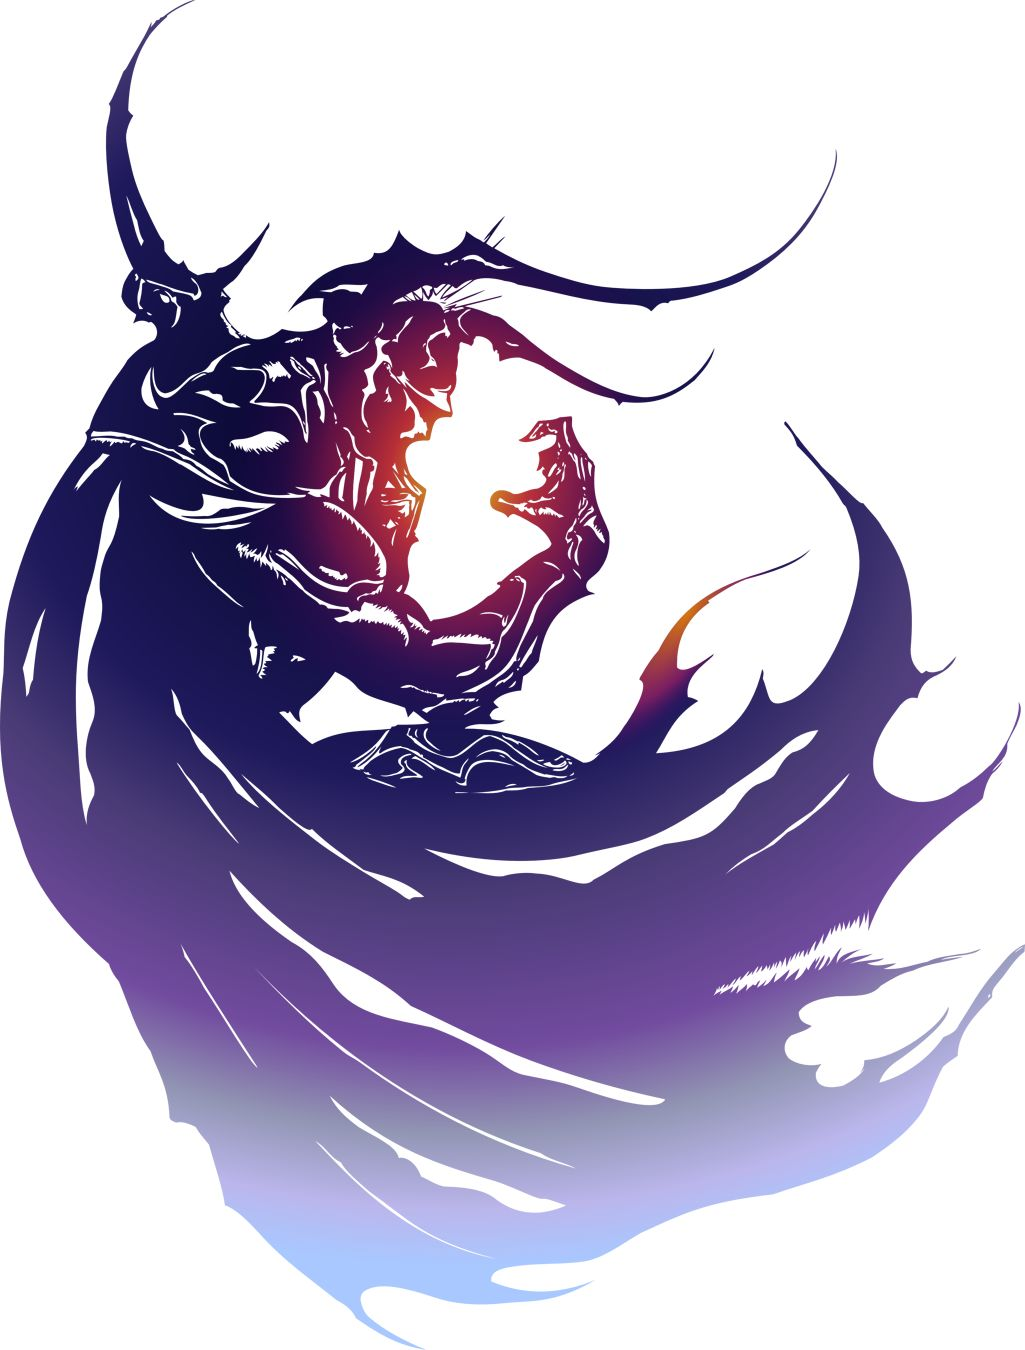
\includegraphics[width=\columnwidth]{./art/images/ff4.jpg} \\\\
%
%
%\vfill
%
%Most adventures are too long to be completed in a single sitting and have to be divided into multiple \accf{sessions}.
%Therefore, it is sufficient to prepare content only for the next session instead of everything in advance.
%Often, it also makes sense to dedicate the very first session of an adventure on its setup, including an introduction of the setting and the player characters.
%During gameplay, look out for opportunities to gracefully end an ongoing session, for example after the conclusion of a quest.
%Sessions can be planned according to adventure Milestones, where Level ups should occur roughly every one to four sessions.
%Still, you will not be able to prepare for everything, so do not be afraid to improvise when necessary.
%%
%\newpage
%%
%\accf{Checks} are a powerful tool that help you to decide the outcome of uncertain actions.
%When players attempt actions you can ask them for checks by assigning a secret DC to the task.
%In some situations you can also proactively ask players to make checks, for example to decide whether the party notices an ambush.
%All non-player characters controlled by you may also have to do checks, as they follow the same rules.
%However, you can refrain from using checks whenever the outcome of an action is reasonably clear.
%%
%\ofpar
%%
%\ofboxwithtitle{Example: Using Checks}{
%	Zidane and Blank try to deliver a convincing staged sword fight to an audience of nobles.
%	The GM decides that this is difficult (DC 9), because the nobles have high expectations. 
%	Zidane rolls 2d with the result 9, so he barely passes the check. 
%	The GM decides that most of the nobles are happy with the delivered performance, but Queen Brahme is not impressed. 
%}
%%
%\ofpar
%%
%Also note that you have two tools to modify checks: \accf{(Dis)advantage} and \accf{Fortune Dice}. 
%Giving Advantage on a check allows you to express that the odds are unusually in the favor of the actor, for example because he is very well prepared or has help from another character. 
%In contrast, Disadvantage usually implies that something is actively working against him, which could be a natural circumstance but also a particularly clumsy or unsuitable approach to the problem by the actor.
%In comparison, Fortune Dice allow the party to benefit from random luck in some situations, but suffer from misfortune in others.
%While players can use them to improve their odds in crucial moments, you can use them to create dramatic and unexpected moments.
%For example, while the party is running away from their pursuers, they perform a check to avoid an obstacle on the ground and you can use a low Fortune Die to make sure that a characters trips. 
%Will the rest of the party help their friend and be confronted with the pursuers or will they leave him behind and return to save him later?
%%
%\ofpar
%%
%The players can get familiar with the world, by \accf{exploring} different locations.
%However, travelling on foot is often not the best choice due to difficult terrain, weather or ambushes.
%Depending on the setting, more comfortable forms of transportation might be available such as ships, trains, airships, cars or Chocobos.
%Usually, the party needs to employ such a service, but as they become more wealthy, they may acquire their own vehicles.
%For longer journeys, keep track of the amount of time that passes, which also affects the rest of the world.
%\accf{Time} often passes at a different speed in the game than at your table, because uneventful aspects of the adventure can be narrated quickly, while important decisions need to be thought through more carefully.
%To immerse yourself and the players into your world, it is also helpful to give short, vivid descriptions of the party's current surroundings.
%In doing so, focus on elements that could be interesting for the players to interact with.
%Likewise, picture the descriptions given by players about their character's actions to create your narrations of the outcome.
%This often requires you to take the role of many different characters yourself to interact with the party.
%In that case, understand the perspective of the character to portray how they would talk and act when confronted with the party.
%%
%\ofpar
%%
%\ofboxwithtitle{Example: Narrating \& Roleplaying\vspace*{0.2cm}}
%{
%	\acc{Yasumi (Game Master):}
%	As you enter Riovannes Castle, you find yourself inside a large hall with narrow water streams running on both sides.
%	Among multiple dead knights that lie scattered on the ground, you can see a man standing at the end of the central stairway.
%	He turns around and you realize it is none other than Wiegraf Folles! \vspace{0.25cm}\\
%	\acc{Yasumi (playing as Wiegraf):} There you are Ramza. Draw your sword. \vspace{0.25cm}\\			
%	\acc{Akihiko:} I don't draw my sword yet. Maybe we can solve this peacefully. \vspace{0.25cm}\\	
%	\acc{Yasumi (playing as Wiegraf):} What's wrong? If you don't, I will. \vspace{0.25cm}\\			
%	\acc{Akihiko (playing as Ramza):} How miserable you are. Giving away your spirit just to avenge yourself. \vspace{0.25cm}\\
%	\acc{Yasumi (playing as Wiegraf):} Revenge? That's not what I'm after.
%	I want to bring chaos into the world... But, don't worry. I'll kill you myself! \vspace{0.25cm}\\			
%	\acc{Akihiko:} OK, NOW I definitely draw my sword! \vspace{0.25cm}\\
%	\acc{Yasumi:} Alright, you can take the first turn.
%}
%%
%\ofpar
%%
%%
%\vfill
%%
%Although adventurers spend most of their time on the road, they may sometimes rest for extended periods in towns and villages.
%During this \accf{Downtime}, characters may, aside from resting, pursue a number of side activities.
%You do not need to play this out in detail, instead you can quickly narrate downtime portions.
%Usually, it is sufficient to assign a cost and a time frame to the activities, but for particularly difficult tasks you can also ask the player for a check to decide whether he can successfully complete it.
%The list below gives some generic examples of such downtime activities and their approximate costs and durations.
%%
%\\\\
%%
%\oftable{p{0.6\columnwidth} r r}
%{\accf{Downtime Activity} & \accf{Cost} & \accf{Time}}
%{
%	Build a small house & 5000G & weeks \ofrow
%	Build a boat or carriage & 1500G & \ofrow
%	Learn a simple skill (e.g. cooking or sewing) & 250G & a week \ofrow
%	Help locals with simple tasks (e.g. harvest) & 0G & a week \ofrow
%	Send a letter or messenger & 100G & a day \ofrow
%	Attend a local festivity & 50G & a day \ofrow
%	Build a platonic relationship & 10G & a week \ofrow
%	Conduct research (e.g. on a location or person) & 100G & days \ofrow
%	Craft a simple tool or gadget (e.g. an axe or watch) & 200G & days \ofrow
%	Explore the local area & 0G & a day \ofrow
%	Write a book & 100G & weeks \ofrow
%}
%%
%\clearpage
%%
%\ofquote{"World very simple place. World only have two things: things you can eat and things you no can eat."\\}{Quina}\\
%%
%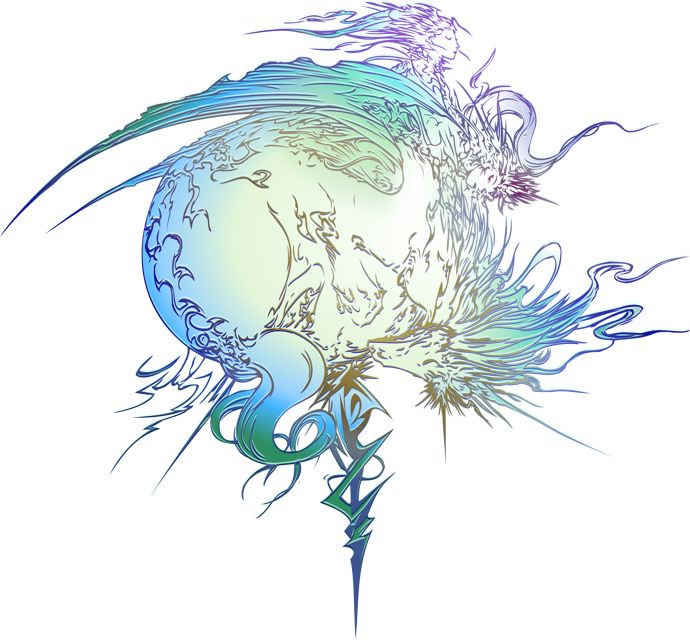
\includegraphics[width=\columnwidth]{./art/images/ff13.jpg}
%%
%\\\\
%%
%Creating a \accf{World} is one of the most difficult, but also most rewarding parts of being a GM.
%The players become part of your world, where they interact with the environment and change it through their actions and decisions. 
%Therefore, you can catch their interest by offering engaging content that allows for meaningful choices.
%Most adventures revolve around a \accf{Central Conflict}, which the party aims to solve as the goal of their adventure.
%Usually, this conflict involves multiple forces with opposing interests and the adventurers can be part of either of these sides.
%Accordingly, there is also an opposing side, a common enemy or antagonist that acts against the party.
%As the GM, you take the role of characters on different sides of this conflict, so you need to consider their different perspectives. 
%%
%\ofpar
%%
%A good way to start building an adventure is to establish what the world looks like on a \accf{Map}. 
%Begin by creating its natural layout including landmasses, water, forests, mountains and deserts. 
%Afterwards, place and mark locations that could be interesting for players to visit, like cities, dungeons or ruins.
%Then add more detail only to the places that the players will likely visit in the beginning, you can do the rest later on.
%You may provide the players with this map at some point in the game to make them aware of these locations you have created.
%After creating some detailed locations, think about who might live in these places.
%These \accf{Non-Player Characters} are roleplayed by you when interacting with the party.
%They live their own lives, independent of the players and have their own personalities, goals, abilities and outlooks on life. 
%Accordingly, they often have knowledge about the world that the players do not.
%They can be allied, neutral or enemies of the party depending on the circumstances.
%For creating detailed non-player characters, you can use the standard character creation rules, but usually it is sufficient to write down some notes about them.
%%
%\ofpar
%%
%In general, the rules try to make as few assumptions as possible to allow for greater freedom in world building.
%Nevertheless, some fantasy elements are deeply ingrained into the game such as \accf{Magic}, Monsters and Espers.
%As such, think about the role they take in your world, but you can feel free to interpret them in your own way.
%For magic it is important to establish its sources, for example in Final Fantasy games, crystals are often portrayed as powerful magic sources and are thus at the center of many conflicts.
%The portrayal of Espers can vary greatly, as they sometimes appear as god-like beings, but in other instances they are interpreted as a mortal race.
%In contrast, monsters take a similar role as wild animals, but just as Espers, they are usually connected to the sources of magic and thus are able to make use of its powers.
%Finally, even though we assume the existence of these magical elements, we give no restrictions concerning their prevalence, so magic in your world can be pervasive and ubiquitous, but it could also be rare and alien.
%%
%\vfill
%%
%Another important aspect that shapes your world is the progression of \accf{Technology}.
%Different technologies, such as machines, vehicles and weapons can complement the magical forces in the world, but may also stand in conflict against them.
%Thus, the societies of your world may prefer or rely on magic and technology to varying degrees in their daily lives.
%However, the lines between these two forces can sometimes be blurry, after all, sufficiently advanced technology is indistinguishable from magic.
%During their adventure, the party can make use of available technologies and might even contribute to the current state of art.
%%
%\vfill
%%
%\ofboxwithtitle{Example: Worldbuilding}
%{
%	The world we create consists two parts: Pulse and Cocoon.
%	Pulse is a huge uncharted planet with a vast nature that is home to various monsters.
%	In contrast, Cocoon is a small planet that floats above Pulse and is inhabited by an advanced human society.
%	The Cocoon citizen depend on the god-like beings for necessities such as food and electricity.
%	These powerful beings are called fal'Cie and can directly or indirectly assert control over humans.
%	The fal'Cie of Cocoon stand in conflict against the fal'Cie of Pulse and accordingly humans are conditioned to be hostile towards Pulse.		
%	Our adventure starts on Cocoon, where an ancient Pulse fal'Cie has been discovered some days ago.
%	In a radical answer, the Cocoon government orders the deportation of all humans that have been near the Pulse fal'Cie.
%	Small rebellion groups form among the citizen to fight back against this so-called "Purge".
%}
%%
%\clearpage
%
%\ofquote{"Wait, he says... Do I look like a waiter?"\\}{Kefka}\\\\
%
Compared to the players, who play the game from the perspective of the protagonists, the \accf{Game Master} has a different role.
He creates the world and setting of the adventure and takes the role of all non-player characters.
Furthermore, the GM describes the environment and narrates the outcomes of all actions. 
Unlike the players, the GM is not bound by strict rules and may make his own rulings when necessary.
There is no single way to be a successful GM and we encourage you adopt a style that is enjoyable for both you and the players.
%
\vfill
%
Accordingly, this chapter does not focus on presenting rules or advice.
Instead, it is a collection of modular \accf{supplements}, that you can either use directly or regard as examples for creating your own content.
These supplements not only to give a glimpse into the various aspects of game mastering, but also show some of the different directions that you can take with Omega Fantasy. 
The present modules can be broadly split into two categories: \accf{prepared content} and \accf{rule changes}.
The former provide you with world building blocks such as adventures, settings and monsters that are self-contained and extensible.
The latter present you examples to customize the rules to your preferences.
While the prepared content is well suited for beginners, we recommend to consider rule changes once you have gathered some experience with Omega Fantasy.
All available supplements are listed in the following, together with a short synopsis for each one.
%
\newpage
%
\accf{Bestiary:} this section discusses guidelines for creating interesting monsters and combat encounters.
Furthermore, it includes a large collection of prepared enemies that you can either directly use for you game or regard as examples for creating your own ones.
%
\vfill
%
\accf{Chaos in Cornelia:} a short adventure in which the party has to save a kidnapped princess. 
Highly recommended for beginners and provides an easy entry into Omega Fantasy.
Contains diverse content covering different aspects of adventuring, such as combat, roleplaying and exploration.
%
\vfill
%
\accf{Tomb of Raithwall:} a short adventure in which the party has to recover an ancient artifact from a dangerous tomb.
Focused on exploring a challenging environment where traps and adversaries may lurk around every corner. 
%
\vfill
%
\accf{Maria \& Draco:} a single-session adventure in which the party has to ensure the success of an opera performance.
Encourages a more light-hearted narrative with a focus on interesting roleplaying moments.
%
\vfill
%
\accf{Siege of Dollet:} a single-session adventure in which the party has to pass a practical test to join an elite mercenary force.
Focuses on creating an action packed narrative with multiple combat encounters.
%
\vfill
%
\accf{Gold Saucer:} an amusement park where the party can blow off steam and win rare prizes. 
This one is more loosely structured and focuses on recreating the various games in the park, which can serve you as an example on how to create non-combat competitions.  
%
\vfill
%
\accf{Ivalice Worldbook:} a very detailed document focused on fleshing out the world of Ivalice, including its history and geography.
This helps you to create various adventures in this world, but it can also serve as an example of how to create a detailed setting.
%
\vfill
%
\accf{Optional Rules:} minor rule changes and additions that help you to customize the feeling of the game.
%
\vfill
%
\accf{Races:} rules and examples for incorporating different humanoid races in your world. 
This provides additional character creation options for players, but can also help you to create a more interesting game world.
%
\vfill
%
\accf{Chocobos:} rules for incorporating bird-like creatures called Chocobos as full-fledged party members.
Players can raise Chocobos, use them as mounts and fight alongside them in combat.
%
\vfill
%
\accf{Triple Triad:} rules for a fun card game, allowing the party to collect and play cards.
Well suited if you are looking quick and simple side-activity for the party.
%
\vfill
%
\accf{Blitzball:} rules for a fun team-based sports game similar to water polo.
Well suited if you are looking for a more elaborate side-activity for the party.
%
\vfill
%
\accf{Filled Character Sheets:} sheets for Level~1 characters that you or the players can directly use or regard as examples for creating your own.
%
\clearpage



